\section{CUDA}\label{sec:CUDA}

\textbf{CUDA} is a parallel computing platform and programming model by NVIDIA that exposes GPUs for general-purpose computing. It provides the core infrastructure to accelerate compute-intensive algorithms, such as matrix multiplication, by distributing the parallel workload across thousands of cores.
The specific CUDA architectural parameters and capabilities utilized in this implementation correspond to the hardware configurations previously detailed in the GPU Hardware Specifications (Section~\ref{sec:GPU spec}). 

\paragraph{CUDA Hierarchy and Execution Model}
The CUDA programming model structures execution through a three-tiered hardware abstraction hierarchy. A kernel invocation from the host instantiates a \textbf{grid} on the device, which is partitioned into independent \textbf{blocks}. Each block encapsulates up to 1024 concurrent \textbf{threads}. Crucially, threads within the same block can synchronize execution and share data via low-latency \textbf{Shared Memory (SMEM)}.

The spatial topology of this hierarchy is defined by the built-in \texttt{dim3} vector types: \texttt{blockDim} determines the thread layout per block, bounded by the architectural limit $$\text{blockDim.x} \times \text{blockDim.y} \times \text{blockDim.z} \leq 1024$$
Consequently, \texttt{gridDim} defines the number of allocated blocks in the grid.

\paragraph{Kernel execution}
In this section we will test different kernels, executed with custom function \emph{launch\_kernel} whose goal is simply to define the grid and the block's size: 

\begin{lstlisting}[style=CStyle, caption={Example code to launch the Naive Kernel: the block's sizes can be defined at runtime. }, label={lst:cuda_launch_kernel}]
extern int cu_block_x, cu_block_y;

void launch_kernel(int n, m_type *dA, m_type *dB, m_type *dC) {
    dim3 block(cu_block_x, cu_block_y);
    dim3 grid(CEIL_DIV(n, cu_block_x), CEIL_DIV(n, cu_block_y));
    kernel<<<grid, block>>>(n, dA, dB, dC);
}
\end{lstlisting}

What happens: 
\begin{itemize}
    \item \texttt{dim3 block(cu\_block\_x, cu\_block\_y)}: defines the dimension of each thread block
    \begin{itemize}
        \item Example: $16 \times 16 = 256$ threads per block
    \end{itemize}
    \item \texttt{dim3 grid(...)}: defines how many blocks are needed to cover the entire matrix
    \item \texttt{kernel<<<grid, block>>>}: CUDA syntax to launch the kernel
    \begin{itemize}
        \item \texttt{grid}: grid configuration
        \item \texttt{block}: block configuration
    \end{itemize}
\end{itemize}
The dimensions of the thread block can be dynamically defined at runtime, allowing for the adjustment of \texttt{cu\_block\_x} and \texttt{cu\_block\_y}.

\paragraph{Experimental methodology}
The CUDA development involved the implementation of various kernel types, starting from the simplest version, defined as \emph{naive}, and then proceeding with increasingly optimized versions, each one fixing the limitations of the previous iteration.

The recorded execution times for the various tests reflect not only the actual matrix multiplication, but also GPU memory allocation for the matrices, data transfers between the host (CPU) and the device (GPU) including the resulting matrix, GPU memory deallocation, and the CUDA kernel launch overhead.
All tests were performed using matrices of size $N = 15000$ to study performance consistently across all implemented kernel types.

\subsection{Kernel 1: Naive Implementation}


For the first kernel, we leverage the \textbf{grid, block, and thread} hierarchy to uniquely assign each thread to a single element of the resulting matrix $C$. This structure allows each thread to compute the dot product of a row from $A$ and a column from $B$ in total autonomy.

\begin{lstlisting}[style=CStyle, caption={Naive CUDA matrix multiplication kernel}, label={lst:cuda_naive_kernel}]
__global__ void kernel(int n, const m_type *A, const m_type *B, m_type *C) {
    int row = blockIdx.y * blockDim.y + threadIdx.y;
    int col = blockIdx.x * blockDim.x + threadIdx.x;
    if (row < n && col < n) {
        m_type sum = 0.0;
        for (int t = 0; t < n; ++t) {
            sum += A[row * n + t] * B[t * n + col];
        }
        C[row * n + col] = sum;
    }
}
\end{lstlisting}

The kernel invocation is handled according to the logic defined in Listing \ref{lst:cuda_launch_kernel}. To optimize performance on a matrix of size \textbf{N=15000}, a runtime hyperparameter optimization phase was performed, focusing on the parameters \textbf{\texttt{cu\_block\_x}
} and \textbf{\texttt{cu\_block\_y}}. This procedure allowed a systematic analysis of the impact of their combinations on execution time. 
The different combinations studied are from powers of two, starting from 2 and going up to 1024.

\begin{figure}[H]
    \centering
    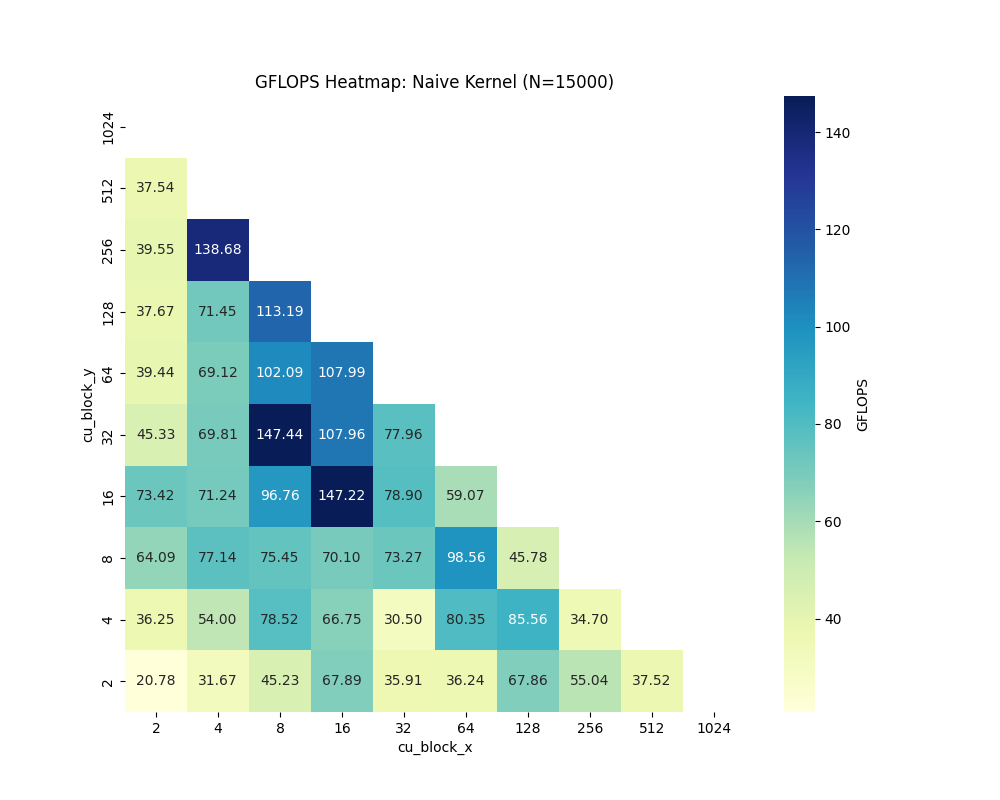
\includegraphics[width=0.8\textwidth]{Images/naive_heatmap.png}
    \caption{HeatMap of hyper-parameter tuning on a matrix $n = 15000$}
    \label{fig:orig_tune_t}
\end{figure} 

\paragraph{Performance Analysis} In the CUDA architecture, instructions are processed in \textbf{warps}, indivisible hardware units of 32 threads operating in SIMT mode. Maximum performance is achieved by saturating the resources of the Streaming Multiprocessors (SMs) and avoiding warp divergence, i.e., idle threads caused by the execution of a heterogeneous set of instructions within the threads of a warp.
\begin{itemize}
    \item \textbf{Optimal Performance:} The best performance (147.4 GFLOPS) is achieved with block sizes of 8x32 and 16x16, both generating 256 threads per block. The two kernels exhibit very similar performance and can therefore be considered equivalent, as the minor discrepancy between the two values is negligible due to measurement noise. This size is optimal because it perfectly aligns with the GPU's hardware limitations, allowing it to activate the maximum possible number of concurrent threads. With a high number of active operations, the hardware effectively masks memory access latencies. 
    
    Additionally, the GPU executes instructions in indivisible groups of 32 threads (warps). Since 256 is a perfect multiple of 32, each warp is completely filled and no computational power is wasted.

\begin{table}[h]
\centering
\begin{tabular}{rrrr}
\toprule
cu\_block\_x & cu\_block\_y & seconds & gflops \\
\midrule
8 & 32 & 45.779 & 147.44 \\
16 & 16 & 45.848 & 147.22 \\
\bottomrule
\end{tabular}
\caption{Best possible performance of the naive kernel (8x32  and 16x16)}
\label{tab:optimal_blocks_perf}
\end{table}

\item \textbf{Worst Performance:} Conversely, the $2 \times 2$ configuration yields the worst performance (20.8 GFLOPS), generating only 4 threads per block. The GPU imposes a physical limit on the number of blocks it can schedule concurrently. 

For example, in the architecture used for this project, the Streaming Multiprocessor (SM) can handle a maximum of 16 blocks simultaneously. If each block contains only 4 threads, the maximum number of active threads per SM will be: $16 \text{ blocks} \times 4 \text{ threads} = 64 \text{ active threads}$. Thus, given a hardware limit of 1024 threads per SM, exactly 6.25\% (64/1024) of the available computing capacity is utilized, leaving the remainder idle. Consequently, this causes a severe waste of resources.

\begin{table}[h]
\centering
\begin{tabular}{rrrr}
\toprule
cu\_block\_x & cu\_block\_y & seconds & gflops \\
\midrule
2 & 2 & 324.519 & 20.80 \\
\bottomrule
\end{tabular}
\caption{Worst possible performance of the naive kernel (2x2)}
\label{tab:worst_perf}
\end{table}

\item \textbf{Hardware Limits (Empty areas):} The cells lacking data represent configurations where the product of $cu\_block\_x \times cu\_block\_y$ exceeds the maximum hardware limit of 1024 threads per block. Such configurations violate architectural constraints, physically preventing the kernel launch.

\end{itemize}

\paragraph{Observation :} Despite both configurations using 256 threads, the $8 \times 32$ block doubles the performance compared to the $32 \times 8$ one ($ 147.4$ GFLOPS vs. $ 73.3$ GFLOPS) due to the different organization of threads within the warp. Since the hardware groups threads by columns, in a $32 \times 8$ block, a warp covers an entire row, forcing the GPU to perform 32 distinct fetches from Global Memory for each iteration. 

In contrast, in the $8 \times 32$ block, the warp folds across 4 rows and 8 columns: threads on different rows reuse the same 8 elements of matrix B already present in memory, drastically reducing latency and doubling efficiency.


\paragraph{Kernel Register Pressure}
To verify the above claims, the flags \texttt{-Xptxas -v} were used to analyze the register pressure specific to the NVIDIA T4 architecture using the naive kernel; the output shows:

\begin{quote}
    \texttt{0 bytes stack frame, 0 bytes spill stores, 0 bytes spill loads \\
    ptxas info : Used 63 registers, used 0 barriers, 384 bytes cmem[0]}
\end{quote}

\begin{itemize}
    \item \textbf{0 bytes spill stores/loads}: Indicates the absence of register spilling. This certifies that the execution does not suffer from bottlenecks due to spilling temporary data into high-latency local memory.
    \item \textbf{Used 63 registers}: Each thread allocates 63 physical registers. On the \textbf{sm\_75} architecture, which features a Register File of \textbf{65,536 registers} per Streaming Multiprocessor (SM), this configuration allows the scheduler to allocate up to 1024 concurrent threads (e.g., 4 blocks of 256). 
    
    Since the total demand ($63 \times 1024 = 64,512$) remains within the physical limit, the hardware successfully saturates the \textbf{theoretical occupancy at 100\%} without inducing register spilling.
    \item \textbf{used 0 barriers}: The kernel does not invoke hardware barrier primitives.
    \item \textbf{Absence of smem data}: The shared memory value is completely absent because the naive approach does not explicitly use it. Each thread performs direct loads from the Global Memory (VRAM). Since there are no arrays declared in the code with the \texttt{\_\_shared\_\_} qualifier, the compiler does not reserve any space in the on-chip shared memory portion.
\end{itemize}

\paragraph{NvProf Analysis} Based on the identified optimal parameters $16 \times 16$ ,equal to the performance 8x32, we will now proceed with a performance profiling analysis using \texttt{nvprof} to examine the kernel behavior in detail taking into account only a few of the most important parameters.

\begin{table}[h]
\centering
\begin{tabular}{lrr}
\toprule
Name & Time (\%) & Time \\
\midrule
\texttt{[CUDA memcpy HtoD]} & 1.61 & 755.88ms \\
\texttt{[CUDA memcpy DtoH]} & 0.80 & 377.45ms \\
\texttt{cudaDeviceSynchronize} & 96.96 & 45.7910s \\
\texttt{cudaMemcpy} & 2.40 & 1.13479s \\
\texttt{cudaMalloc} & 0.61 & 290.09ms \\
\texttt{cudaFree} & 0.01 & 5.9084ms \\
\bottomrule
\end{tabular}
\caption{Nvprof Analysis for Naive Kernel with block 16x16}
\label{tab:nvprof_memory_sync}
\end{table}

\textbf{GPU Activities:}
\begin{itemize}
    \item \texttt{[CUDA memcpy HtoD]} (1.61\% - 755.88ms): Represents the physical transfer of the two operand matrices ($A$ and $B$) from system RAM to GPU VRAM. The execution of two calls justifies a time exactly double that of the inverse operation.
    \item \texttt{[CUDA memcpy DtoH]} (0.80\% - 377.45ms): Transfer of the single result matrix from VRAM to RAM.
\end{itemize}

\textbf{API Calls:}
\begin{itemize}
    \item \texttt{cudaDeviceSynchronize} (96.96\% - 45.79s): It is the explicit barrier point. The time recorded in this API exactly coincides with the kernel execution time: the CPU remains in a blocked state waiting for the device to empty the asynchronous execution queue.
    \item \texttt{cudaMemcpy} (2.40\% - 1.13s): Host-side overhead for orchestrating synchronous transfers.
    \item \texttt{cudaMalloc} (0.61\% - 290.09ms): Computational cost to map and allocate the three matrices in the global address space (VRAM).
    \item \texttt{cudaFree} (0.01\% - 5.9ms): VRAM deallocation operation at the end of the cycle.
\end{itemize}


\paragraph{Limitations and Resume}
Concluding the analysis of this kernel, since \textit{tiling} is missing (which we will see implemented in the next kernel), \textit{Shared Memory} is neither exploited nor used in this kernel. Consequently, the same element of matrix B is read from \textit{Global Memory} multiple times, saturating the memory with redundant data requests. Finally, by computing only a single element of matrix C per thread (each iteration must read and update the same \texttt{sum} accumulator), the GPU fails to overlap multiple mathematical instructions to mask hardware latencies.


\subsection{Kernel 2: Tiling}
A new kernel is introduced that uses the concept of tiling. Tiling is an optimization technique present in CUDA kernels that consists of dividing matrices into smaller blocks (tiles). Each tile is processed separately, often loading the data into shared memory to reduce global memory access costs. 

This allows for better exploitation of data locality and parallelism, improving performance compared to element-by-element processing.
\paragraph{Kernel Call}
The Tiling kernel uses a compile-time constant \texttt{TILE\_WIDTH} to ensure a square geometry. In contrast, the Naive kernel uses run-time parameters because, by not implementing shared memory, it has no allocation constraints and allows dynamic adjustment of the block topology to optimize memory usage. In the Tiling kernel, static shared memory allocation is architecturally necessary so that the compiler can determine the exact memory footprint of each thread block \textit{a priori}.
\begin{lstlisting}[style=CStyle, caption={Code to launch Kernel 2}, label={lst:cuda_coalesced_kernel}]
void launch_kernel(int n, m_type *dA, m_type *dB, m_type *dC) {
    dim3 block(TILE_WIDTH, TILE_WIDTH);
    dim3 grid((n + TILE_WIDTH - 1)/TILE_WIDTH, (n + TILE_WIDTH - 1)/TILE_WIDTH);
    kernel<<<grid, block>>>(n, dA, dB, dC);
}
\end{lstlisting}
\paragraph{Kernel Code}The code performs matrix multiplication on the GPU exploiting the tiling technique, where each thread block works on a portion, called a tile, of the matrix. The data of matrices $A$ and $B$ are loaded into the shared memory of the block, allowing faster access compared to global memory.

Each thread computes an element of the resulting matrix $C$, accumulating the product of the corresponding elements within the tile. Synchronization among the threads occurs via \texttt{\_\_syncthreads()} to ensure that all data are correctly loaded and used. At the end of the computation, the result is written to matrix $C$ only if the thread is within the limits of the matrix. 

\begin{lstlisting}[style=CStyle, caption={CUDA implementation of Kernel 2}, label={lst:Kernel_2_code}]
__global__ void kernel(int n, const m_type *A, const m_type *B, m_type *C) {
    int bx = blockIdx.x, by = blockIdx.y;
    int tx = threadIdx.x, ty = threadIdx.y;

    int row = by * TILE_WIDTH + ty;
    int col = bx * TILE_WIDTH + tx;

    __shared__ m_type sA[TILE_WIDTH][TILE_WIDTH];
    __shared__ m_type sB[TILE_WIDTH][TILE_WIDTH];

    m_type sum = 0.0;
    int numTiles = (n + TILE_WIDTH - 1) / TILE_WIDTH;

    for (int m = 0; m < numTiles; ++m) {
        if (row < n && m * TILE_WIDTH + tx < n)
            sA[ty][tx] = A[row * n + m * TILE_WIDTH + tx];
        else
            sA[ty][tx] = 0.0;

        if (m * TILE_WIDTH + ty < n && col < n)
            sB[ty][tx] = B[(m * TILE_WIDTH + ty) * n + col];
        else
            sB[ty][tx] = 0.0;

        __syncthreads();

        for (int k = 0; k < TILE_WIDTH; ++k) {
            sum += sA[ty][k] * sB[k][tx];
        }

        __syncthreads();
    }

    if (row < n && col < n) {
        C[row * n + col] = sum;
    }
}
\end{lstlisting}

\paragraph{Performance Analysis} Before beginning the analysis of the results, it is important to note that the maximum \texttt{TILE\_WIDTH} value depends on the shared memory available per block and the number of threads. On NVIDIA T4 GPUs, each block can use up to 64 KB of shared memory, but typically only 48 KB is allocated by default for static allocations. This means that \texttt{TILE\_WIDTH} must be chosen so that the memory required by the blocks falls within this limit, taking into account both the number of threads and the data type used. Furthermore, performance was studied by performing multiple iterations for each test to analyze whether there were any discrepancies between the results. Five different iterations were performed for each experiment conducted.

\begin{itemize}
    \item \textbf{\texttt{First Experiment ( 32 x 32 ):}} Kernel 2 clearly surpasses the performance of Kernel 1, exceeding 200~GFLOPS. By exploiting Data Reuse in Shared Memory, fetches from Global Memory are drastically reduced, freeing bandwidth on the bus and masking access latency. 

    \begin{table}[H]
    \centering
    \begin{tabular}{ccc}
    \toprule
    \texttt{TILE\_WIDTH} & Time (s) & GFLOPS \\
    \midrule
    32 & 31.509 & 214.22 \\
    32 & 32.027 & 210.76 \\
    32 & 32.498 & 207.70 \\
    32 & 32.782 & 205.91 \\
    32 & 33.022 & 204.41 \\
    \bottomrule
    \end{tabular}
    \caption{Kernel Performance using 32 x 32}
    \label{tab:kernel2_15000}
    \end{table}
    
    Furthermore, the footprint of a $32 \times 32$ block in double precision requires only 16~KB of Shared Memory (the calculation is: $2 \times (32 \times 32) \times 8 \text{ bytes} = 16,384 \text{ bytes} = 16 \text{ KB}$): falling well within the 48~KB limit of T4 GPUs, it allows the scheduler to allocate more blocks for each Streaming Multiprocessor. 
    
    From the results, however, a variance in execution times can be noted: although the root cause is not clear, a progressive performance decay is evident in the iterations following the first one.
    

    \item \textbf{\texttt{Second Experiment ( 16 x 16 ):}} In the second case where a 16x16 dimension was used, we can notice a drop in GFLOPS, from 214.22 to 197.14. 

    \begin{table}[H]
    \centering
    \begin{tabular}{ccc}
    \toprule
    \texttt{TILE\_WIDTH} & Time (s) & GFLOPS \\
    \midrule
    16 & 34.239 & 197.14 \\
    16 & 35.232 & 191.59 \\
    16 & 36.069 & 187.14 \\
    16 & 36.769 & 183.58 \\
    16 & 37.186 & 181.52 \\
    \bottomrule
    \end{tabular}
    \caption{Kernel Performance using 16 x 16}
    \label{tab:kernel_16x16}
    \end{table}
    
    This is attributable to the lower data reuse. In the Tiling technique, each element loaded from the slower Global Memory to the faster Shared Memory is reused for calculations a number of times equal to the dimension of the tile itself (\texttt{TILE\_WIDTH}). 
    
    With a $32 \times 32$ tile, each fetch in Global Memory is reused 32 times, while with a $16 \times 16$ tile, the same fetch is reused only 16 times. As previously stated for the $32 \times 32$ kernel, a performance degradation can be observed between iterations.


    \item \textbf{\texttt{Third Experiment:}}Following the analysis of the different tile dimensions and the progressive performance degradation observed between iterations, a further test was conducted on the $16 \times 16$ kernel, recording a drastic drop in GFLOPS compared to the previous measurement. 

    \begin{table}[H]
    \centering
    \begin{tabular}{ccc}
    \toprule
    \texttt{TILE\_WIDTH} & Time (s) & GFLOPS \\
    \midrule
    16 & 36.969 & 182.58 \\
    16 & 39.715 & 169.96 \\
    16 & 40.752 & 165.64 \\
    16 & 40.367 & 167.21 \\
    16 & 40.493 & 166.69 \\
    \bottomrule
    \end{tabular}
    \caption{Kernel Performance using 16 x 16 (Repeated)}
    \label{tab:kernel_16x16_final}
    \end{table}
    
\end{itemize}

\paragraph{Note: Cloud Execution Variance} 
As a general comment on the testing methodology, it is crucial to address the high variance and progressive performance degradation observed across iterations in all experiments. Because the Google Colab execution environment operates strictly as a black box, it is impossible to predict, thoroughly understand, or systematically test the root causes of these fluctuations.

Despite keeping the kernel code and execution parameters strictly unchanged, execution times vary significantly between independent tests (some tests had variability of more than $10\%$). This erratic behavior is entirely subdued by Colab's opaque hardware scheduler and its dynamic allocation of shared cloud resources, placing the exact cause of the degradation entirely beyond the scope of user control or local analysis.

    
\paragraph{Kernel Register Pressure}Can see that compared to previous kernels we can notice a different output

\begin{quote}
\texttt{0 bytes stack frame, 0 bytes spill stores, 0 bytes spill loads \\
ptxas info    : Used 42 registers, used 1 barriers, 16384 bytes smem, 384 bytes cmem[0]}
\end{quote}
\begin{itemize}
    \item \textbf{Register Pressure (42 vs 63 registers):} Register usage decreases compared to Kernel 1. The introduction of Shared Memory simplifies the arithmetic for calculating vector indices and reduces the temporary variables active at runtime, significantly lowering the pressure on the Register File.
    \item \textbf{Shared Memory (16384 bytes smem):} The memory footprint confirms the geometric configuration \texttt{TILE\_WIDTH = 32}. The exact calculation is $2 \times (32 \times 32 \times 8 \text{ bytes}) = 16384 \text{ bytes}$ of static shared memory for the two tiles. 
    
    In previous kernels, this parameter was null due to direct access to Global Memory.

    
    \item \textbf{Synchronization (1 barrier):} The PTX compiler reports the allocation of a single hardware barrier at the block level (corresponding to \texttt{\_\_syncthreads()}). This forces the stall of the warps, ensuring that all threads have completed fetching data into Shared Memory before starting arithmetic operations.
\end{itemize}
\vspace{20px}

\paragraph{Nvprof Analysis} Here are the results of using Kernel 32x32 :
\begin{table}[h]
\centering
\begin{tabular}{lrr}
\toprule
Name & Time (\%) & Time \\
\midrule
\texttt{[CUDA memcpy HtoD]} & 2.59 & 780.14ms \\
\texttt{[CUDA memcpy DtoH]} & 1.28 & 386.85ms \\
\texttt{cudaDeviceSynchronize} & 95.46 & 29.0082s \\
\texttt{cudaMemcpy} & 3.85 & 1.16866s \\
\texttt{cudaMalloc} & 0.65 & 197.03ms \\
\texttt{cudaFree} & 0.02 & 6.0008ms \\
\bottomrule
\end{tabular}
\caption{Nvprof Analysis of Kernel 2}
\label{tab:nvprof_analysis_updated}
\end{table}

\begin{itemize}
    \item \texttt{cudaDeviceSynchronize}: In the naive kernel, the kernel completion wait time stabilized at 45.79 seconds. In Kernel Tiling, however, the value dropped to 29.00 seconds. This demonstrates the effectiveness of shared memory.
    \item \texttt{[CUDA memcpy HtoD]} and \texttt{[CUDA memcpy DtoH]}: The absolute times for data transfers from device to host and vice versa remain almost constant between the two versions. The tiling optimization acts solely on the access pattern to the GPU internal memory, not altering the volume of data exchanged between Host and Device.
    \item \texttt{cudaMemcpy}: The slight increase is a direct consequence of the physical time increment of HtoD/DtoH.
    \item The remaining values remained practically unchanged.
\end{itemize}

\subsection{Final Comparison} 

As a final baseline test, the \textbf{cuBLAS} library was employed to establish peak achievable performance. As observed, with the exception of very small workloads, this implementation performs significantly better than all previous custom kernels.

\begin{table}[H]
\centering
\resizebox{\textwidth}{!}{%
  \begin{threeparttable}
    \caption{CUDA Kernel's performance comparison. Percentages reflect computational throughput (GFLOPS) relative to the cuBLAS baseline.}
    \label{tab:final_cublas_comparison_selected}
    \begin{tabular}{l|ccc|ccc|ccc|ccc}
    \toprule
     & \multicolumn{3}{c|}{\textbf{N = 1000}} & \multicolumn{3}{c|}{\textbf{N = 5000}} & \multicolumn{3}{c|}{\textbf{N = 10000}} & \multicolumn{3}{c}{\textbf{N = 15000}} \\
    \textbf{Implementation} & \textbf{Time (s)} & \textbf{GFLOPS} & \textbf{\%} & \textbf{Time (s)} & \textbf{GFLOPS} & \textbf{\%} & \textbf{Time (s)} & \textbf{GFLOPS} & \textbf{\%} & \textbf{Time (s)} & \textbf{GFLOPS} & \textbf{\%} \\
    \midrule
    Kernel 1 (16x16) & 0.330 & 6.06 & 121.82\% & 1.600 & 156.25 & 82.88\% & 11.034 & 181.26 & 80.85\% & 42.411 & 159.16 & 69.10\% \\
    Kernel 2 (32x32) & 0.307 & 6.51 & 130.94\% & 1.411 & 177.18 & 93.98\% & 9.973  & 200.54 & 89.45\% & 33.582 & 201.00 & 87.26\% \\
    \midrule
    \textbf{cuBLAS}  & \textbf{0.402} & \textbf{4.98} & \textbf{100.00\%} & \textbf{1.326} & \textbf{188.54} & \textbf{100.00\%} & \textbf{8.921} & \textbf{224.19} & \textbf{100.00\%} & \textbf{29.304} & \textbf{230.34} & \textbf{100.00\%} \\
    \bottomrule
    \end{tabular}
  \end{threeparttable}%
}
\end{table}

Analyzing the table, it is evident that for very small values of $N$ (such as $N = 1000$), overall performance is poor; notably, the \textbf{cuBLAS} implementation underperforms compared to Kernel 2 despite its theoretical superiority. 
This stems from GPU inefficiency under heavily reduced workloads, where setup latency significantly exceeds effective computation time. Kernel launch and data management introduce fixed overheads that, for small matrices, account for nearly the entire execution duration. 

Rather than a strict application of Amdahl's Law, this bottleneck is primarily dictated by extremely low GPU occupancy. Insufficient thread block generation fails to saturate the available Streaming Multiprocessors (SMs), meaning the hardware cannot effectively use warp scheduling to hide memory access and launch latencies, making the operation a victim of system overhead.

Concluding the analysis, an asymptotic flattening of the throughput curve is observed for Kernel 2 (tiling) and cuBLAS as workloads scale up. Kernel 1, however, scales reasonably well only up to $N = 10000$ (reaching 181.25~GFLOPS), after which it suffers a severe efficiency collapse. At $N = 15000$ and beyond, Kernel 1 regresses from over 80\% down to roughly 69\% of the cuBLAS baseline. Since the naive algorithm lacks \textit{data reuse} optimization, each thread is forced to repeatedly fetch operands directly from Global Memory. 

As the matrix size grows, this dynamic rapidly saturates the memory bus bandwidth, inducing severe memory stalls in the Streaming Multiprocessors. Because all warps are eventually forced to wait on memory transactions, the SM scheduler is unable to swap active warps to hide the latency. Unlike Kernel 1, Kernel 2 demonstrates significantly superior architectural stability by leveraging Shared Memory to bypass the memory wall, ensuring excellent overall performance, albeit confined just below the maximum limit achieved by the highly optimized cuBLAS routines.


